\section{Actors}
\label{actor}

Actors in \lib are a lightweight abstraction for units of computations. They
are active objects in the sense that they own their state and do not allow
others to access it. The only way to modify the state of an actor is sending
messages to it.

\lib provides several actor implementations, each covering a particular use
case. The available implementations differ in three characteristics: (1)
dynamically or statically typed, (2) class-based or function-based, and (3)
using asynchronous event handlers or blocking receives. These three
characteristics can be combined freely, with one exception: statically typed
actors are always event-based. For example, an actor can have dynamically typed
messaging, implement a class, and use blocking receives. The common base class
for all user-defined actors is called \lstinline^local_actor^.

Dynamically typed actors are more familiar to developers coming from Erlang or
Akka. They (usually) enable faster prototyping but require extensive unit
testing. Statically typed actors require more source code but enable the
compiler to verify communication between actors. Since CAF supports both,
developers can freely mix both kinds of actors to get the best of both worlds.
A good rule of thumb is to make use of static type checking for actors that are
visible across multiple translation units.

Actors that utilize the blocking receive API always require an exclusive thread
of execution. Event-based actors, on the other hand, are usually scheduled
cooperatively and are very lightweight with a memory footprint of only few
hundred bytes. Developers can exclude---detach---event-based actors that
potentially starve others from the cooperative scheduling while spawning it. A
detached actor lives in its own thread of execution.

\subsection{Environment / Actor Systems}
\label{actor-system}

All actors live in an \lstinline^actor_system^ representing an actor
environment including scheduler~\see{scheduler}, registry~\see{registry}, and
optional components such as a middleman~\see{middleman}. A single process can
have multiple \lstinline^actor_system^ instances, but this is usually not
recommended (a use case for multiple systems is to strictly separate two or
more sets of actors by running them in different schedulers). For configuration
and fine-tuning options of actor systems see \sref{system-config}. A
distributed CAF application consists of two or more connected actor systems. We
also refer to interconnected \lstinline^actor_system^ instances as a
\emph{distributed actor system}.

\clearpage
\subsection{Common Actor Base Types}

The following pseudo-UML depicts the class diagram for actors in \lib.
Irrelevant member functions and classes as well as mixins are omitted for
brevity. Selected individual classes are presented in more detail in the
following sections.

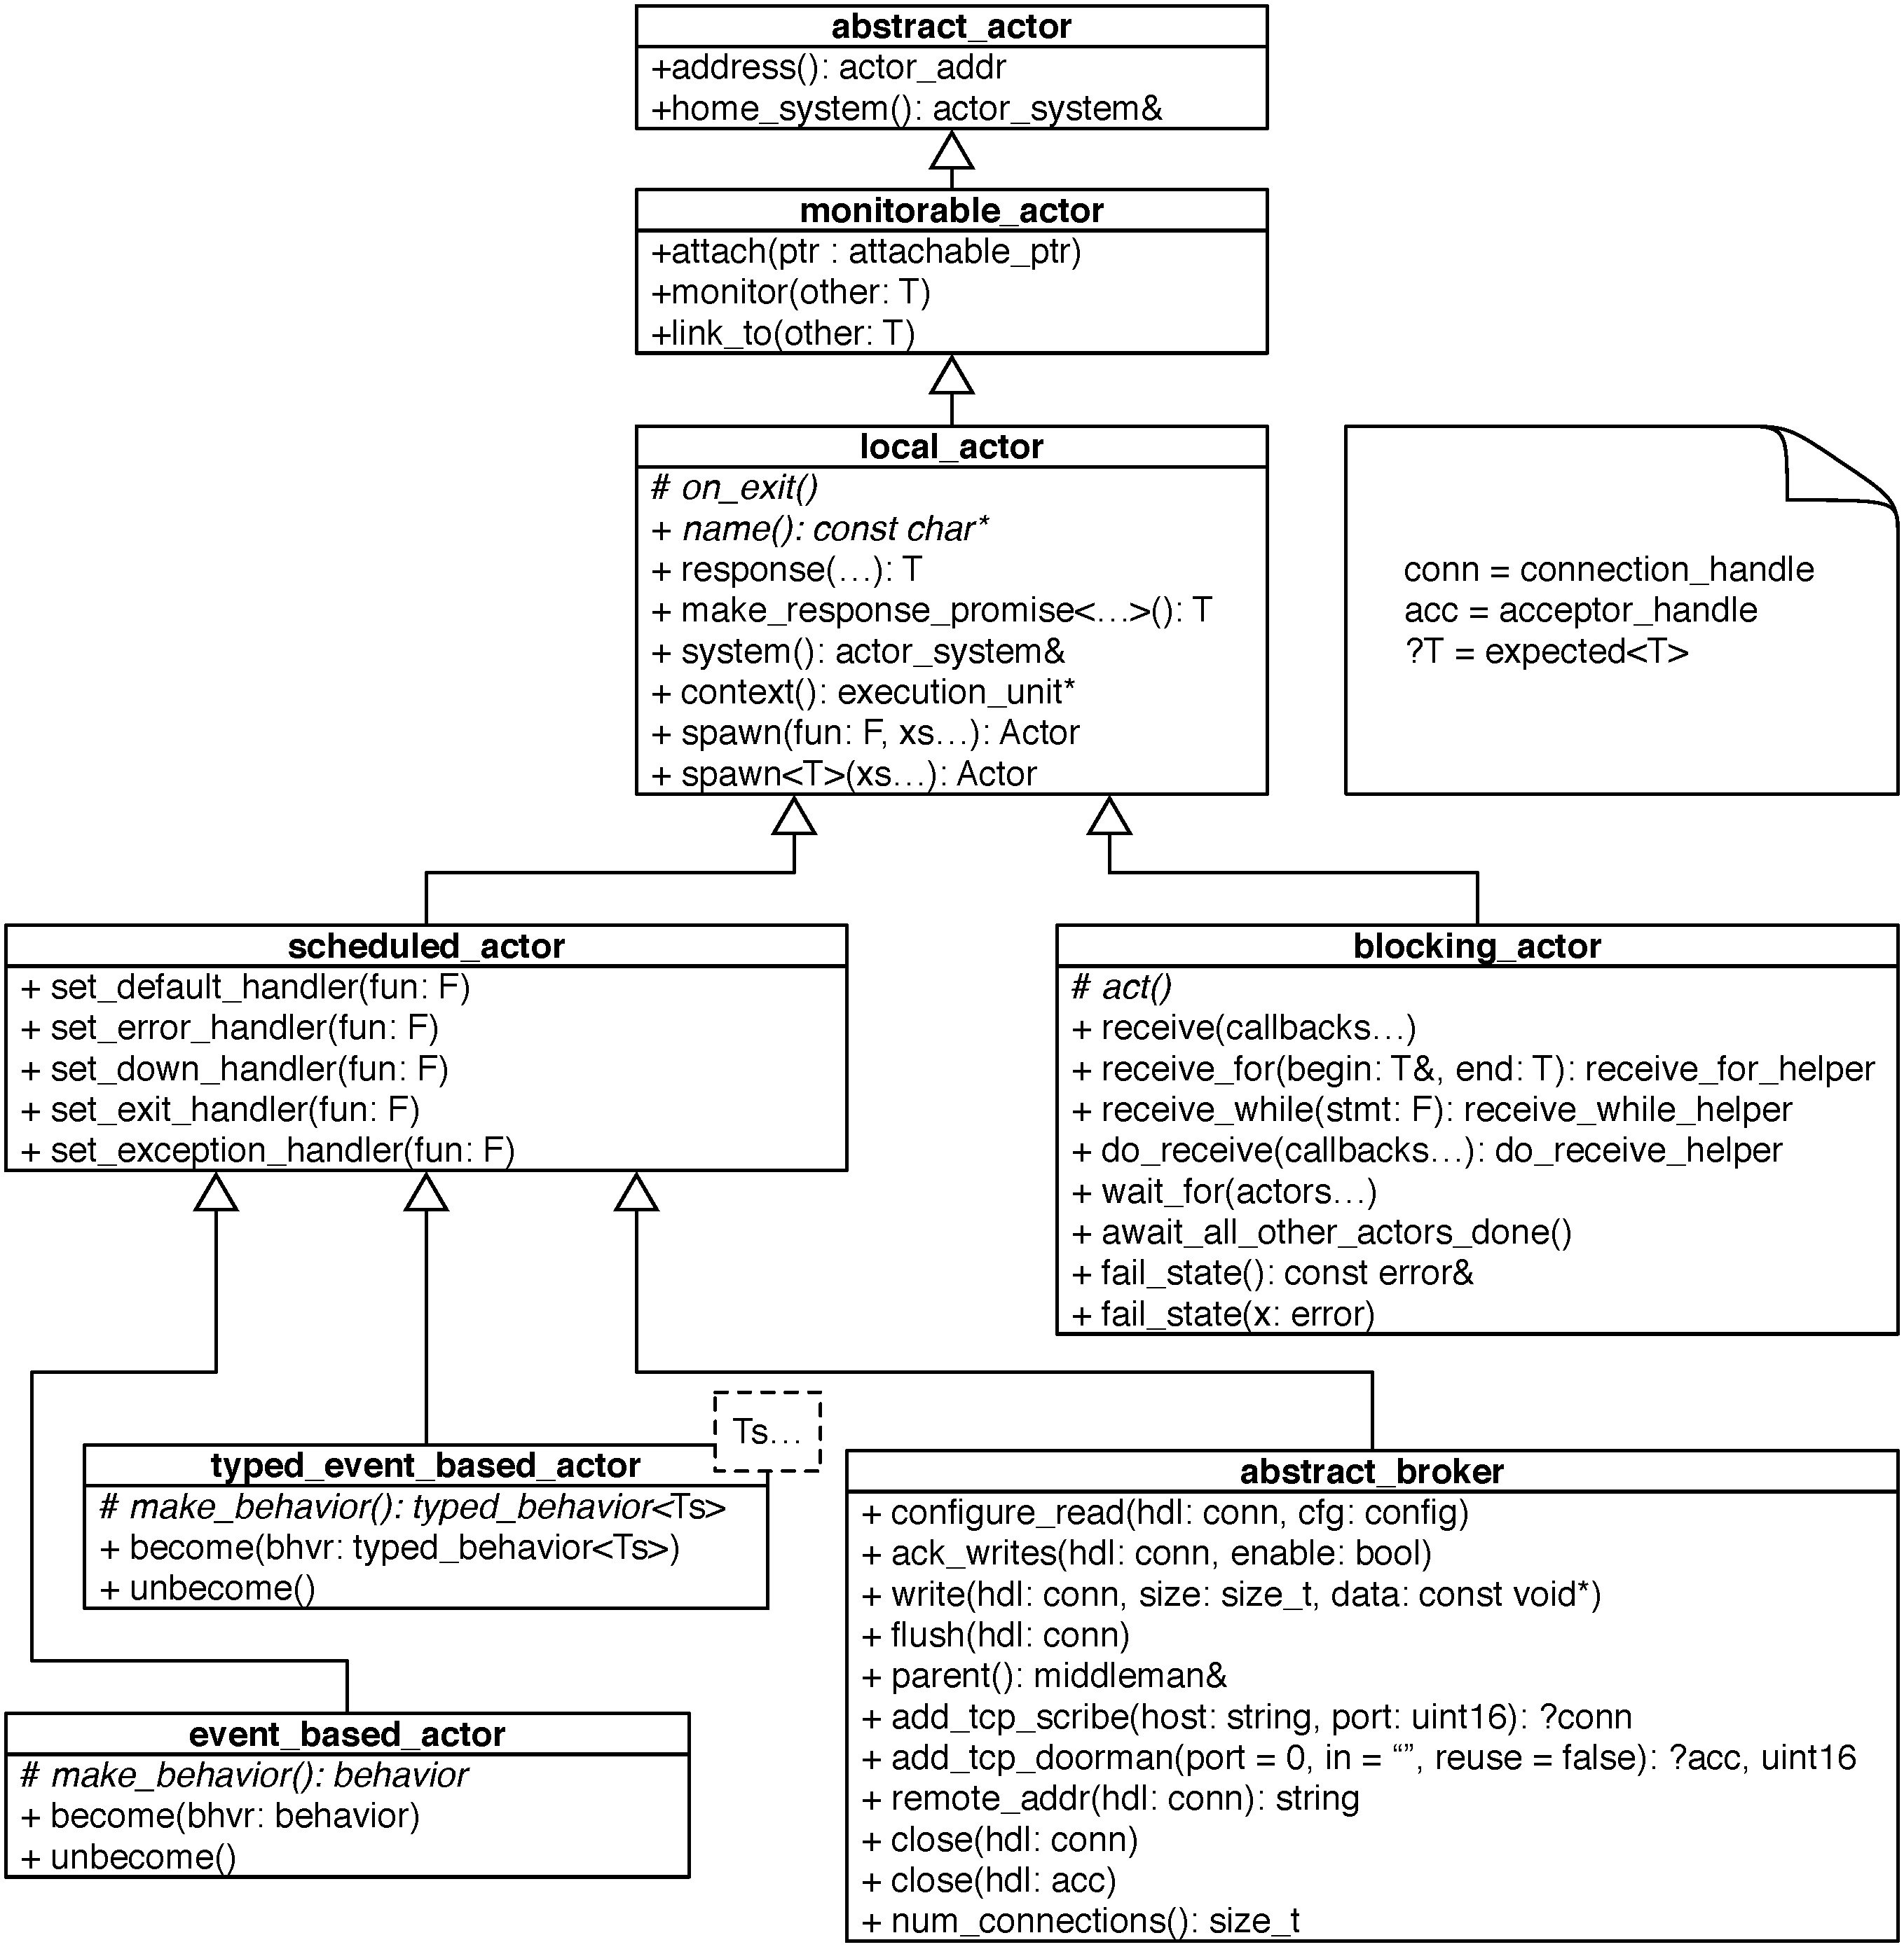
\includegraphics[width=\textwidth]{actor_types}

\clearpage
\subsubsection{Class \lstinline^local_actor^}

The class \lstinline^local_actor^ is the root type for all user-defined actors
in \lib. It defines all common operations. However, users of the library
usually do not inherit from this class directly. Proper base classes for
user-defined actors are \lstinline^event_based_actor^ or
\lstinline^blocking_actor^. The following table also includes member function
inherited from \lstinline^monitorable_actor^ and \lstinline^abstract_actor^.

\begin{center}
\begin{tabular}{ll}
  \textbf{Types} & ~ \\
  \hline
  \lstinline^mailbox_type^ & A concurrent, many-writers-single-reader queue type. \\
  \hline
  ~ & ~ \\ \textbf{Constructors} & ~ \\
  \hline
  \lstinline^(actor_config&)^ & Constructs the actor using a config. \\
  \hline
  ~ & ~ \\ \textbf{Observers} & ~ \\
  \hline
  \lstinline^actor_addr address()^ & Returns the address of this actor. \\
  \hline
  \lstinline^actor_system& system()^ & Returns \lstinline^context()->system()^. \\
  \hline
  \lstinline^actor_system& home_system()^ & Returns the system that spawned this actor. \\
  \hline
  \lstinline^execution_unit* context()^ & Returns underlying thread or current scheduler worker. \\
  \hline
  ~ & ~ \\ \textbf{Customization Points} & ~ \\
  \hline
  \lstinline^on_exit()^ & Can be overridden to perform cleanup code. \\
  \hline
  \lstinline^const char* name()^ & Returns a debug name for this actor type. \\
  \hline
  ~ & ~ \\ \textbf{Actor Management} & ~ \\
  \hline
  \lstinline^link_to(other)^ & Link to an actor \see{link}. \\
  \hline
  \lstinline^unlink_from(other)^ & Remove link to an actor \see{link}. \\
  \hline
  \lstinline^monitor(other)^ & Unidirectionally monitors an actor \see{monitor}. \\
  \hline
  \lstinline^demonitor(other)^ & Removes a monitor from \lstinline^whom^. \\
  \hline
  \lstinline^spawn(F fun, xs...)^ & Spawns a new actor from \lstinline^fun^. \\
  \hline
  \lstinline^spawn<T>(xs...)^ & Spawns a new actor of type \lstinline^T^. \\
  \hline
  ~ & ~ \\ \textbf{Message Processing} & ~ \\
  \hline
  \lstinline^T make_response_promise<Ts...>()^ & Allows an actor to delay its response message. \\
  \hline
  \lstinline^T response(xs...)^ & Convenience function for creating fulfilled promises. \\
  \hline
\end{tabular}
\end{center}

\clearpage
\subsubsection{Class \lstinline^scheduled_actor^}

All scheduled actors inherit from \lstinline^scheduled_actor^. This includes
statically and dynamically typed event-based actors as well as brokers
\see{broker}.

\begin{center}
\begin{tabular}{ll}
  \textbf{Types} & ~ \\
  \hline
  \lstinline^pointer^ & \lstinline^scheduled_actor*^ \\
  \hline
  \lstinline^exception_handler^ & \lstinline^function<error (pointer, std::exception_ptr&)>^ \\
  \hline
  \lstinline^default_handler^ & \lstinline^function<result<message> (pointer, message_view&)>^ \\
  \hline
  \lstinline^error_handler^ & \lstinline^function<void (pointer, error&)>^ \\
  \hline
  \lstinline^down_handler^ & \lstinline^function<void (pointer, down_msg&)>^ \\
  \hline
  \lstinline^exit_handler^ & \lstinline^function<void (pointer, exit_msg&)>^ \\
  \hline
  ~ & ~ \\ \textbf{Constructors} & ~ \\
  \hline
  \lstinline^(actor_config&)^ & Constructs the actor using a config. \\
  \hline
  ~ & ~ \\ \textbf{Termination} & ~ \\
  \hline
  \lstinline^quit()^ & Stops this actor with normal exit reason. \\
  \hline
  \lstinline^quit(error x)^ & Stops this actor with error \lstinline^x^. \\
  \hline
  ~ & ~ \\ \textbf{Special-purpose Handlers} & ~ \\
  \hline
  \lstinline^set_exception_handler(F f)^ & Installs \lstinline^f^ for converting exceptions to errors \see{error}. \\
  \hline
  \lstinline^set_down_handler(F f)^ & Installs \lstinline^f^ to handle down messages \see{down-message}. \\
  \hline
  \lstinline^set_exit_handler(F f)^ & Installs \lstinline^f^ to handle exit messages \see{exit-message}. \\
  \hline
  \lstinline^set_error_handler(F f)^ & Installs \lstinline^f^ to handle error messages (see \sref{error-message} and \sref{error}). \\
  \hline
  \lstinline^set_default_handler(F f)^ & Installs \lstinline^f^ as fallback message handler \see{default-handler}. \\
  \hline
\end{tabular}
\end{center}

\clearpage
\subsubsection{Class \lstinline^blocking_actor^}

A blocking actor always lives in its own thread of execution. They are not as
lightweight as event-based actors and thus do not scale up to large numbers.
The primary use case for blocking actors is to use a \lstinline^scoped_actor^
for ad-hoc communication to selected actors. Unlike scheduled actors, \lib does
\textbf{not} dispatch system messages to special-purpose handlers. A blocking
actors receives \emph{all} messages regularly through its mailbox. A blocking
actor is considered \emph{done} only after it returned from \lstinline^act^ (or
from the implementation in function-based actors). A \lstinline^scoped_actor^
sends its exit messages as part of its destruction.

\begin{center}
\begin{tabular}{ll}
  \textbf{Constructors} & ~ \\
  \hline
  \lstinline^(actor_config&)^ & Constructs the actor using a config. \\
  \hline
  ~ & ~ \\ \textbf{Customization Points} & ~ \\
  \hline
  \lstinline^void act()^ & Implements the behavior of the actor. \\
  \hline
  ~ & ~ \\ \textbf{Termination} & ~ \\
  \hline
  \lstinline^const error& fail_state()^ & Returns the current exit reason. \\
  \hline
  \lstinline^fail_state(error x)^ & Sets the current exit reason. \\
  \hline
  ~ & ~ \\ \textbf{Actor Management} & ~ \\
  \hline
  \lstinline^wait_for(Ts... xs)^ & Blocks until all actors \lstinline^xs...^ are done. \\
  \hline
  \lstinline^await_all_other_actors_done()^ & Blocks until all other actors are done. \\
  \hline
  ~ & ~ \\ \textbf{Message Handling} & ~ \\
  \hline
  \lstinline^receive(Ts... xs)^ & Receives a message using the callbacks \lstinline^xs...^. \\
  \hline
  \lstinline^receive_for(T& begin, T end)^ & See \sref{receive-loop}. \\
  \hline
  \lstinline^receive_while(F stmt)^ & See \sref{receive-loop}. \\
  \hline
  \lstinline^do_receive(Ts... xs)^ & See \sref{receive-loop}. \\
  \hline
\end{tabular}
\end{center}

\clearpage
\subsection{Messaging Interfaces}
\label{interface}

Statically typed actors require abstract messaging interfaces to allow the
compiler to type-check actor communication. Interfaces in CAF are defined using
the variadic template \lstinline^typed_actor<...>^, which defines the proper
actor handle at the same time. Each template parameter defines one
\lstinline^input/output^ pair via
\lstinline^replies_to<X1,...,Xn>::with<Y1,...,Yn>^. For inputs that do not
generate outputs, \lstinline^reacts_to<X1,...,Xn>^ can be used as shortcut for
\lstinline^replies_to<X1,...,Xn>::with<void>^. In the same way functions cannot
be overloaded only by their return type, interfaces cannot accept one input
twice (possibly mapping it to different outputs). The example below defines a
messaging interface for a simple calculator.

\cppexample[17-21]{message_passing/calculator}

It is not required to create a type alias such as \lstinline^calculator_actor^,
but it makes dealing with statically typed actors much easier. Also, a central
alias definition eases refactoring later on.

Interfaces have set semantics. This means the following two type aliases
\lstinline^i1^ and \lstinline^i2^ are equal:

\begin{lstlisting}
using i1 = typed_actor<replies_to<A>::with<B>, replies_to<C>::with<D>>;
using i2 = typed_actor<replies_to<C>::with<D>, replies_to<A>::with<B>>;
\end{lstlisting}

Further, actor handles of type \lstinline^A^ are assignable to handles of type
\lstinline^B^ as long as \lstinline^B^ is a subset of \lstinline^A^.

For convenience, the class \lstinline^typed_actor<...>^ defines the member
types shown below to grant access to derived types.

\begin{center}
\begin{tabular}{ll}
  \textbf{Types} & ~ \\
  \hline
  \lstinline^behavior_type^ & A statically typed set of message handlers. \\
  \hline
  \lstinline^base^ & Base type for actors, i.e., \lstinline^typed_event_based_actor<...>^. \\
  \hline
  \lstinline^pointer^ & A pointer of type \lstinline^base*^. \\
  \hline
  \lstinline^stateful_base<T>^ & See \sref{stateful-actor}. \\
  \hline
  \lstinline^stateful_pointer<T>^ & A pointer of type \lstinline^stateful_base<T>*^. \\
  \hline
  \lstinline^extend<Ts...>^ & Extend this typed actor with \lstinline^Ts...^. \\
  \hline
  \lstinline^extend_with<Other>^ & Extend this typed actor with all cases from \lstinline^Other^. \\
  \hline
\end{tabular}
\end{center}

\clearpage
\subsection{Spawning Actors}
\label{spawn}

Both statically and dynamically typed actors are spawned from an
\lstinline^actor_system^ using the member function \lstinline^spawn^. The
function either takes a function as first argument or a class as first template
parameter. For example, the following functions and classes represent actors.

\cppexample[24-29]{message_passing/calculator}

Spawning an actor for each implementation is illustrated below.

\cppexample[140-145]{message_passing/calculator}

Additional arguments to \lstinline^spawn^ are passed to the constructor of a
class or used as additional function arguments, respectively. In the example
above, none of the three functions takes any argument other than the implicit
but optional \lstinline^self^ pointer.

\subsection{Function-based Actors}
\label{function-based}

When using a function or function object to implement an actor, the first
argument \emph{can} be used to capture a pointer to the actor itself. The type
of this pointer is usually \lstinline^event_based_actor*^ or
\lstinline^blocking_actor*^. The proper pointer type for any
\lstinline^typed_actor^ handle \lstinline^T^ can be obtained via
\lstinline^T::pointer^ \see{interface}.

Blocking actors simply implement their behavior in the function body. The actor
is done once it returns from that function.

Event-based actors can either return a \lstinline^behavior^
\see{message-handler} that is used to initialize the actor or explicitly set
the initial behavior by calling \lstinline^self->become(...)^. Due to the
asynchronous, event-based nature of this kind of actor, the function usually
returns immediately after setting a behavior (message handler) for the
\emph{next} incoming message. Hence, variables on the stack will be out of
scope once a message arrives. Managing state in function-based actors can be
done either via rebinding state with \lstinline^become^, using heap-located
data referenced via \lstinline^std::shared_ptr^ or by using the ``stateful
actor'' abstraction~\see{stateful-actor}.

The following three functions implement the prototypes shown in~\sref{spawn}
and illustrate one blocking actor and two event-based actors (statically and
dynamically typed).

\clearpage
\cppexample[31-72]{message_passing/calculator}

\clearpage
\subsection{Class-based Actors}
\label{class-based}

Implementing an actor using a class requires the following:
\begin{itemize}
\item Provide a constructor taking a reference of type
  \lstinline^actor_config&^ as first argument, which is forwarded to the base
    class. The config is passed implicitly to the constructor when calling
    \lstinline^spawn^, which also forwards any number of additional arguments
    to the constructor.
\item Override \lstinline^make_behavior^ for event-based actors and
  \lstinline^act^ for blocking actors.
\end{itemize}

Implementing actors with classes works for all kinds of actors and allows
simple management of state via member variables. However, composing states via
inheritance can get quite tedious. For dynamically typed actors, composing
states is particularly hard, because the compiler cannot provide much help. For
statically typed actors, \lib also provides an API for composable
behaviors~\see{composable-behavior} that works well with inheritance. The
following three examples implement the forward declarations shown in
\sref{spawn}.

\cppexample[74-108]{message_passing/calculator}

\clearpage
\subsection{Stateful Actors}
\label{stateful-actor}

The stateful actor API makes it easy to maintain state in function-based
actors. It is also safer than putting state in member variables, because the
state ceases to exist after an actor is done and is not delayed until the
destructor runs. For example, if two actors hold a reference to each other via
member variables, they produce a cycle and neither will get destroyed. Using
stateful actors instead breaks the cycle, because references are destroyed when
an actor calls \lstinline^self->quit()^ (or is killed externally). The
following example illustrates how to implement stateful actors with static
typing as well as with dynamic typing.

\cppexample[18-44]{message_passing/cell}

Stateful actors are spawned in the same way as any other function-based actor
\see{function-based}.

\cppexample[49-50]{message_passing/cell}

\clearpage
\subsection{Actors from Composable Behaviors \experimental}
\label{composable-behavior}

When building larger systems, it is often useful to implement the behavior of
an actor in terms of other, existing behaviors. The composable behaviors in
\lib allow developers to generate a behavior class from a messaging
interface~\see{interface}.

The base type for composable behaviors is \lstinline^composable_behavior<T>^,
where \lstinline^T^ is a \lstinline^typed_actor<...>^. \lib maps each
\lstinline^replies_to<A,B,C>::with<D,E,F>^ in \lstinline^T^ to a pure virtual
member function with signature:

\begin{lstlisting}
  result<D, E, F> operator()(param<A>, param<B>, param<C>);.
\end{lstlisting}

Note that \lstinline^operator()^ will take integral types as well as atom
constants simply by value. A \lstinline^result<T>^ accepts either a value of
type \lstinline^T^, a \lstinline^skip_t^ \see{default-handler}, an
\lstinline^error^ \see{error}, a \lstinline^delegated<T>^ \see{delegate}, or a
\lstinline^response_promise<T>^ \see{promise}. A \lstinline^result<void>^ is
constructed by returning \lstinline^unit^.

A behavior that combines the behaviors \lstinline^X^, \lstinline^Y^, and
\lstinline^Z^ must inherit from \lstinline^composed_behavior<X,Y,Z>^ instead of
inheriting from the three classes directly. The class
\lstinline^composed_behavior^ ensures that the behaviors are concatenated
correctly. In case one message handler is defined in multiple base types, the
\emph{first} type in declaration order ``wins''. For example, if \lstinline^X^
and \lstinline^Y^ both implement the interface
\lstinline^replies_to<int,int>::with<int>^, only the handler implemented in
\lstinline^X^ is active.

Any composable (or composed) behavior with no pure virtual member functions can
be spawned directly through an actor system by calling
\lstinline^system.spawn<...>()^, as shown below.

\cppexample[20-52]{composition/calculator_behavior}

\clearpage

The second example illustrates how to use non-primitive values that are wrapped
in a \lstinline^param<T>^ when working with composable behaviors. The purpose
of \lstinline^param<T>^ is to provide a single interface for both constant and
non-constant access. Constant access is modeled with the implicit conversion
operator to a const reference, the member function \lstinline^get()^, and
\lstinline^operator->^.

When acquiring mutable access to the represented value, \lib copies the value
before allowing mutable access to it if more than one reference to the value
exists. This copy-on-write optimization avoids race conditions by design, while
minimizing copy operations \see{copy-on-write}. A mutable reference is returned
from the member functions \lstinline^get_mutable()^ and \lstinline^move()^. The
latter is a convenience function for \lstinline^std::move(x.get_mutable())^.
The following example illustrates how to use \lstinline^param<std::string>^
when implementing a simple dictionary.

\cppexample[22-44]{composition/dictionary_behavior}

\subsection{Attaching Cleanup Code to Actors}
\label{attach}

Users can attach cleanup code to actors. This code is executed immediately if
the actor has already exited. Otherwise, the actor will execute it as part of
its termination. The following example attaches a function object to actors for
printing a custom string on exit.

\cppexample[46-50]{broker/simple_broker}

It is possible to attach code to remote actors. However, the cleanup code will
run on the local machine.

\subsection{Blocking Actors}
\label{blocking-actor}

Blocking actors always run in a separate thread and are not scheduled by \lib.
Unlike event-based actors, blocking actors have explicit, blocking
\emph{receive} functions. Further, blocking actors do not handle system
messages automatically via special-purpose callbacks \see{special-handler}.
This gives users full control over the behavior of blocking actors. However,
blocking actors still should follow conventions of the actor system. For
example, actors should unconditionally terminate after receiving an
\lstinline^exit_msg^ with reason \lstinline^exit_reason::kill^.

\subsubsection{Receiving Messages}

The function \lstinline^receive^ sequentially iterates over all elements in the
mailbox beginning with the first. It takes a message handler that is applied to
the elements in the mailbox until an element was matched by the handler. An
actor calling \lstinline^receive^ is blocked until it successfully dequeued a
message from its mailbox or an optional timeout occurs. Messages that are not
matched by the behavior are automatically skipped and remain in the mailbox.

\begin{lstlisting}
self->receive (
  [](int x) { /* ... */ }
);
\end{lstlisting}

\subsubsection{Catch-all Receive Statements}
\label{catch-all}

Blocking actors can use inline catch-all callbacks instead of setting a default
handler \see{default-handler}. A catch-all case must be the last callback
before the optional timeout, as shown in the example below.

\begin{lstlisting}
self->receive(
  [&](float x) {
    // ...
  },
  [&](const down_msg& x) {
    // ...
  },
  [&](const exit_msg& x) {
    // ...
  },
  others >> [](message_view& x) -> result<message> {
    // report unexpected message back to client
    return sec::unexpected_message;
  }
);
\end{lstlisting}

\clearpage
\subsubsection{Receive Loops}
\label{receive-loop}

Message handler passed to \lstinline^receive^ are temporary object at runtime.
Hence, calling \lstinline^receive^ inside a loop creates an unnecessary amount
of short-lived objects. \lib provides predefined receive loops to allow for
more efficient code.

\begin{lstlisting}
// BAD
std::vector<int> results;
for (size_t i = 0; i < 10; ++i)
  receive (
    [&](int value) {
      results.push_back(value);
    }
  );

// GOOD
std::vector<int> results;
size_t i = 0;
receive_for(i, 10) (
  [&](int value) {
    results.push_back(value);
  }
);
\end{lstlisting}

\begin{lstlisting}
// BAD
size_t received = 0;
while (received < 10) {
  receive (
    [&](int) {
      ++received;
    }
  );
} ;

// GOOD
size_t received = 0;
receive_while([&] { return received < 10; }) (
  [&](int) {
    ++received;
  }
);
\end{lstlisting}
\clearpage

\begin{lstlisting}
// BAD
size_t received = 0;
do {
  receive (
    [&](int) {
      ++received;
    }
  );
} while (received < 10);

// GOOD
size_t received = 0;
do_receive (
  [&](int) {
    ++received;
  }
).until([&] { return received >= 10; });
\end{lstlisting}

The examples above illustrate the correct usage of the three loops
\lstinline^receive_for^, \lstinline^receive_while^ and
\lstinline^do_receive(...).until^. It is possible to nest receives and receive
loops.

\begin{lstlisting}
bool running = true;
self->receive_while([&] { return running; }) (
  [&](int value1) {
    self->receive (
      [&](float value2) {
        aout(self) << value1 << " => " << value2 << endl;
      }
    );
  },
  // ...
);
\end{lstlisting}

\subsubsection{Scoped Actors}
\label{scoped-actors}

The class \lstinline^scoped_actor^ offers a simple way of communicating with
CAF actors from non-actor contexts. It overloads \lstinline^operator->^ to
return a \lstinline^blocking_actor*^. Hence, it behaves like the implicit
\lstinline^self^ pointer in functor-based actors, only that it ceases to exist
at scope end.

\begin{lstlisting}
void test(actor_system& system) {
  scoped_actor self{system};
  // spawn some actor
  auto aut = self->spawn(my_actor_impl);
  self->send(aut, "hi there");
  // self will be destroyed automatically here; any
  // actor monitoring it will receive down messages etc.
}
\end{lstlisting}
